%-------------------------------------------------------------------------------
%	EMPIEZA CAPITULO
%-------------------------------------------------------------------------------

\chapter{Compensador Adelanto/Atraso (LR)}

    El concepto de fase surge del análisis del lugar de las raices, al pensar que el angulo que tiene un conjunto de raices complejas conjugadas con respecto al eje real positivo es la fase, es decir, el angulo del fasor. De esta manera, podemos modificar el comportamiento de un sistema agregando dinámicas al sistema ayudandolo a mover el lugar geométrico de las raices hacia donde lo necesitemos.

    El adelanto de fase pues, será un comportamiento demasiado rápido y subamortiguado y el atraso de fase demasiado lento y sobreamortiguado, por lo que agregaremos polos que atraigan el lugar de las raices y que modifiquen la fase para adelantarla (si es un comportamiento demasiado lento o sobreamortiguado) o atrasarla (si es un comportamiento demasiado rapido o subamortiguado).

    Empezaremos considerando el siguiente sistema como base para nuestros calculos:

    \begin{figure}
        \centering
        \resizebox{0.6\textwidth}{!}{
            \tikzstyle{input} = [coordinate]
            \tikzstyle{output} = [coordinate]
            \tikzstyle{block} = [draw, rectangle, minimum height=3em, minimum width=4em]
            \tikzstyle{sum} = [draw, circle]
            \tikzstyle{init} = [pin edge={to-, thin, black}]

            \begin{tikzpicture}[auto, node distance=2cm, >=latex']
                \node [input, name=entrada] {};
                \node [sum, right of=entrada] (suma) {$+$};
                \node [block, right of=suma] (ganancia) {$k$};
                \node [block, right of=ganancia] (planta) {$G(s)$};
                \node [output, right of=planta] (salida) {};
                \node [block, below of=planta] (retro) {$-1$};

                \draw [->] (entrada) -- node[name=u] {$r(s)$} (suma);
                \draw [->] (suma) -- (ganancia);
                \draw [->] (ganancia) -- (planta);
                \draw [->] (planta) -- node[name=y] {$y(s)$} (salida);
                \draw [->] (y) |- (retro);
                \draw [->] (retro) -| (suma);
            \end{tikzpicture}}
        \caption{\label{dia:caa1}Planta con controlador proporcional y realimentación unitaria.}
    \end{figure}

%-------------------------------------------------------------------------------
%	EMPIEZA SECCION
%-------------------------------------------------------------------------------

    \newpage
    \section{Compensador de adelanto de fase}

        Dado el siguiente sistema realimentado:

        \begin{figure}
            \centering
            \resizebox{0.6\textwidth}{!}{
                \tikzstyle{input} = [coordinate]
                \tikzstyle{output} = [coordinate]
                \tikzstyle{block} = [draw, rectangle, minimum height=3em, minimum width=4em]
                \tikzstyle{sum} = [draw, circle]
                \tikzstyle{init} = [pin edge={to-, thin, black}]

                \begin{tikzpicture}[auto, node distance=2cm, >=latex']
                    \node [input, name=entrada] {};
                    \node [sum, right of=entrada] (suma) {$+$};
                    \node [block, right of=suma] (ganancia) {$G_c(s)$};
                    \node [block, right of=ganancia] (planta) {$G(s)$};
                    \node [output, right of=planta] (salida) {};
                    \node [block, below of=planta] (retro) {$-1$};

                    \draw [->] (entrada) -- node[name=u] {$r(s)$} (suma);
                    \draw [->] (suma) -- (ganancia);
                    \draw [->] (ganancia) -- (planta);
                    \draw [->] (planta) -- node[name=y] {$y(s)$} (salida);
                    \draw [->] (y) |- (retro);
                    \draw [->] (retro) -| (suma);
                \end{tikzpicture}}
            \caption{\label{dia:caa2}Planta con compensador y realimentación unitaria.}
        \end{figure}

        Tenemos que el controlador es de la forma:

        \begin{equation}
            G_c(s) = k_c \alpha \frac{Ts + 1}{\alpha T s + 1} = \hat{k}_c \frac{s + \frac{1}{T}}{s + \frac{1}{\alpha T}}
        \end{equation}

        con $k_c > 0$ y $0 < \alpha < 1$.

        Dadas estas condiciones, el lugar de las raíces de los polos y ceros\footnote{El cero atrae el lugar de las raices hacia la izquierda.} agregados se verán como en la figura.

        \begin{figure}
            \centering
            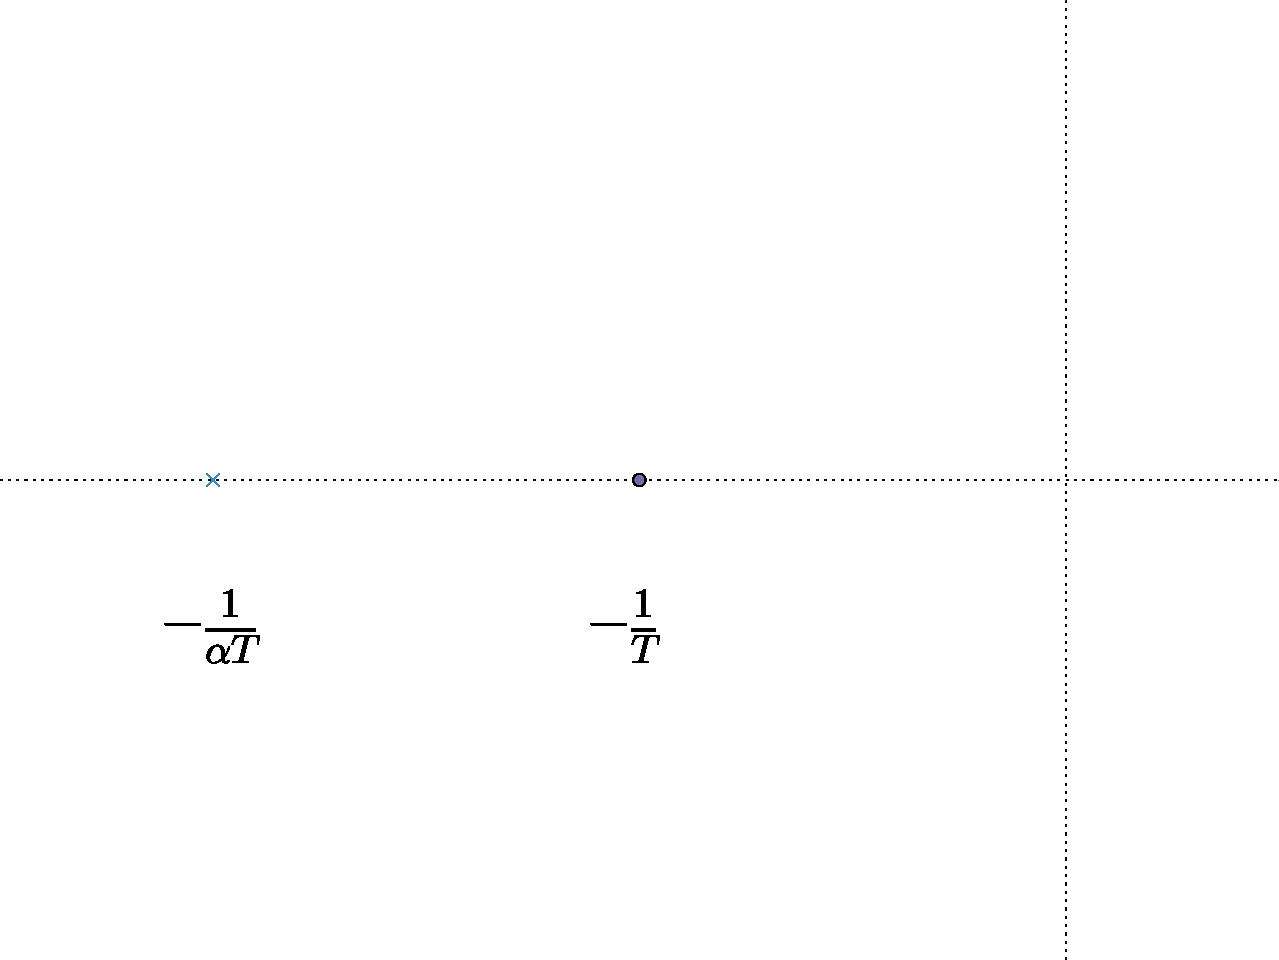
\includegraphics[width=0.7\textwidth]{./imagenes/adelantopoloycero.pdf}
            \caption{\label{fig:adelantopoloycero}Polo y cero introducidos por el compensador de adelanto de fase.}
        \end{figure}

        Dado este controlador se pueden modificar el comportamiento del sistema para hacerlo tan rápido como sea necesario. El calculo de los parametros $T$ y $\alpha$ será explicado con un ejemplo.

%-------------------------------------------------------------------------------

        \subsection{Ejemplo}
        \faltante{Falta escribir apunte}

%-------------------------------------------------------------------------------
%	EMPIEZA SECCION
%-------------------------------------------------------------------------------

    \newpage
    \section{Compensador de atraso de fase}

        Dado el siguiente sistema realimentado:

        \begin{figure}
            \centering
            \resizebox{0.6\textwidth}{!}{
                \tikzstyle{input} = [coordinate]
                \tikzstyle{output} = [coordinate]
                \tikzstyle{block} = [draw, rectangle, minimum height=3em, minimum width=4em]
                \tikzstyle{sum} = [draw, circle]
                \tikzstyle{init} = [pin edge={to-, thin, black}]

                \begin{tikzpicture}[auto, node distance=2cm, >=latex']
                    \node [input, name=entrada] {};
                    \node [sum, right of=entrada] (suma) {$+$};
                    \node [block, right of=suma] (ganancia) {$G_c(s)$};
                    \node [block, right of=ganancia] (planta) {$G(s)$};
                    \node [output, right of=planta] (salida) {};
                    \node [block, below of=planta] (retro) {$-1$};

                    \draw [->] (entrada) -- node[name=u] {$r(s)$} (suma);
                    \draw [->] (suma) -- (ganancia);
                    \draw [->] (ganancia) -- (planta);
                    \draw [->] (planta) -- node[name=y] {$y(s)$} (salida);
                    \draw [->] (y) |- (retro);
                    \draw [->] (retro) -| (suma);
                \end{tikzpicture}}
            \caption{\label{dia:caa3}Planta con ccompensador y realimentación unitaria.}
        \end{figure}

        Tenemos que el controlador es de la forma:

        \begin{equation}
            G_c(s) = k_c \beta \frac{Ts + 1}{\beta T s + 1} = \hat{k}_c \frac{s + \frac{1}{T}}{s + \frac{1}{\beta T}}
        \end{equation}

        con $k_c > 0$ y $\beta > 1$.

        Dadas estas condiciones, el lugar de las raíces de los polos y ceros agregados se verán como en la figura.

        \begin{figure}
            \centering
            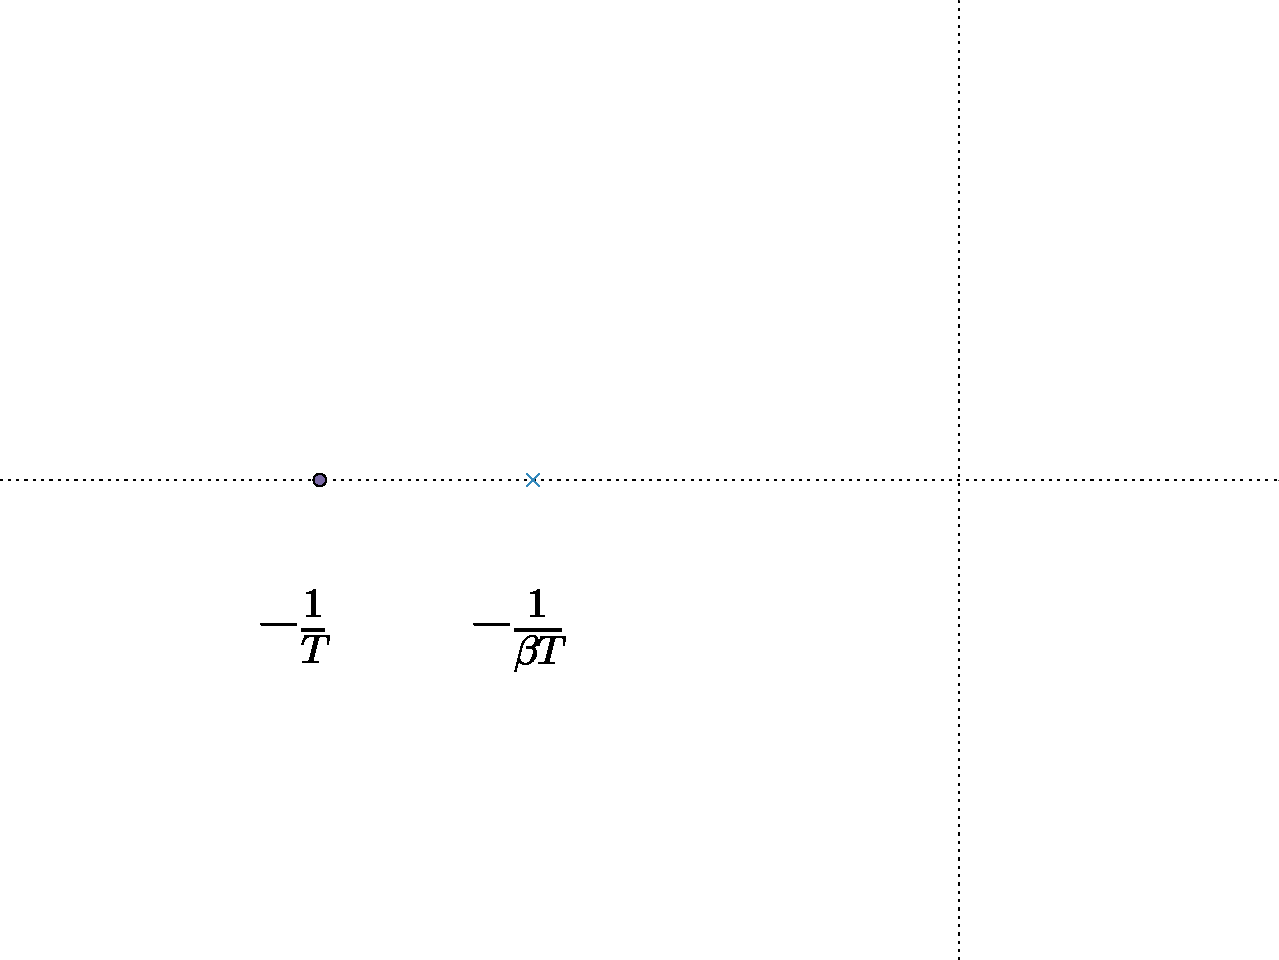
\includegraphics[width=0.7\textwidth]{./imagenes/atrasopoloycero.pdf}
            \caption{\label{fig:atrasopoloycero}Polo y cero introducidos por el compensador de atraso de fase.}
        \end{figure}

        Si el cero y el polo están muy cercanos, entonces para $s=s_1$ un polo dominante en lazo cerrado, se tiene que la magnitud del sistema:

        \begin{equation*}
            \left| G_c(s_1) \right| = \left| \hat{k}_c \frac{s_1 + \frac{1}{T}}{s_1 + \frac{1}{\beta  T}} \right| \approx \left| \hat{k}_c \right|
        \end{equation*}

        y en especifico para la fase:

        \begin{equation*}
            -5^o < \phase{\frac{s_1 + \frac{1}{T}}{s_1 + \frac{1}{\beta  T}}} < 0^o
        \end{equation*}

        Por lo que se puede aumentar la ganancia en el polo del sistema, sin sufrir un corrimiento considerable en el lugar de las raíces.

%-------------------------------------------------------------------------------

        \subsection{Error estático de posición $k_p$}

            Para el sistema dado:

            \begin{figure}
                \centering
                \resizebox{0.6\textwidth}{!}{
                    \tikzstyle{input} = [coordinate]
                    \tikzstyle{output} = [coordinate]
                    \tikzstyle{block} = [draw, rectangle, minimum height=3em, minimum width=4em]
                    \tikzstyle{sum} = [draw, circle]
                    \tikzstyle{init} = [pin edge={to-, thin, black}]

                    \begin{tikzpicture}[auto, node distance=2cm, >=latex']
                        \node [input, name=entrada] {};
                        \node [sum, right of=entrada] (suma) {$+$};
                        \node [block, right of=suma] (planta) {$G(s)$};
                        \node [output, right of=planta] (salida) {};
                        \node [block, below of=planta] (retro) {$-1$};

                        \draw [->] (entrada) -- node[name=u] {$r(s)$} (suma);
                        \draw [->] (suma) -- (planta);
                        \draw [->] (planta) -- node[name=y] {$y(s)$} (salida);
                        \draw [->] (y) |- (retro);
                        \draw [->] (retro) -| (suma);
                    \end{tikzpicture}}
                \caption{\label{dia:caa4}Planta con realimentación unitaria.}
            \end{figure}

            con una entrada de tipo escalón:

            \begin{equation*}
                r(s) = \frac{1}{s}
            \end{equation*}

            y un sistema $G(s)$:

            \begin{equation*}
                G(s) = k_p \frac{s + \frac{1}{T}}{s + \frac{1}{\beta T}}
            \end{equation*}

            El error en estado permanente a una entrada escalón unitario es:

            \begin{equation*}
                e_{ss} = \lim_{s \to 0} s \left( \frac{1}{1 + G(s)} \frac{1}{s} \right) = \lim_{s \to 0} \frac{1}{1 + G(s)} = \frac{1}{1 + G(0)} = \frac{1}{1 + k_p}
            \end{equation*}

            \missingfigure{Gráfica de escalon unitario con error en estado estacionario.}

%-------------------------------------------------------------------------------

        \subsection{Error estático de velocidad $k_v$}
            El error en estado permanente a una entrada rampa unitaria es:

            \begin{equation*}
                r(s) = \frac{1}{s^2}
            \end{equation*}

            \begin{equation*}
                e_{ss} = \lim_{s \to 0} s \left( \frac{1}{a + G(s)} \frac{1}{s^2} \right) = \lim_{s \to 0} \frac{1}{s + s G(s)} = \lim_{s \to 0} \frac{1}{s G(s)} = \frac{1}{k_v}
            \end{equation*}

            \begin{equation*}
                k_v = \lim_{s \to 0} s G(s)
            \end{equation*}

            \missingfigure{Gráfica de rampa unitaria con error en estado estacionario.}

%-------------------------------------------------------------------------------

        \subsection{Ejemplo}
        \faltante{Falta escribir apunte}
